\documentclass[]{elsarticle} %review=doublespace preprint=single 5p=2 column
%%% Begin My package additions %%%%%%%%%%%%%%%%%%%
\usepackage[hyphens]{url}

  \journal{Which journal? Journal of Service Research/Health Services Research/EJOR/IJF} % Sets Journal name


\usepackage{lineno} % add
\providecommand{\tightlist}{%
  \setlength{\itemsep}{0pt}\setlength{\parskip}{0pt}}

\usepackage{graphicx}
\usepackage{booktabs} % book-quality tables
%%%%%%%%%%%%%%%% end my additions to header

\usepackage[T1]{fontenc}
\usepackage{lmodern}
\usepackage{amssymb,amsmath}
\usepackage{ifxetex,ifluatex}
\usepackage{fixltx2e} % provides \textsubscript
% use upquote if available, for straight quotes in verbatim environments
\IfFileExists{upquote.sty}{\usepackage{upquote}}{}
\ifnum 0\ifxetex 1\fi\ifluatex 1\fi=0 % if pdftex
  \usepackage[utf8]{inputenc}
\else % if luatex or xelatex
  \usepackage{fontspec}
  \ifxetex
    \usepackage{xltxtra,xunicode}
  \fi
  \defaultfontfeatures{Mapping=tex-text,Scale=MatchLowercase}
  \newcommand{\euro}{€}
\fi
% use microtype if available
\IfFileExists{microtype.sty}{\usepackage{microtype}}{}
\usepackage[top=25mm, left=30mm, right=30mm, bottom=25mm,headsep=10mm, footskip=12mm]{geometry}
\usepackage{natbib}
\bibliographystyle{plainnat}
\usepackage{longtable}
\ifxetex
  \usepackage[setpagesize=false, % page size defined by xetex
              unicode=false, % unicode breaks when used with xetex
              xetex]{hyperref}
\else
  \usepackage[unicode=true]{hyperref}
\fi
\hypersetup{breaklinks=true,
            bookmarks=true,
            pdfauthor={},
            pdftitle={Short-term hourly forecasting in urgent and emergency care},
            colorlinks=false,
            urlcolor=blue,
            linkcolor=magenta,
            pdfborder={0 0 0}}
\urlstyle{same}  % don't use monospace font for urls

\setcounter{secnumdepth}{5}
% Pandoc toggle for numbering sections (defaults to be off)


% Pandoc header
\usepackage{adjustbox, float}



\begin{document}
\begin{frontmatter}

  \title{Short-term hourly forecasting in urgent and emergency care}
    \author[University1]{Author1\corref{1}}
   \ead{email1@example.com} 
    \author[University2]{Author2\corref{2}}
   \ead{email2@example.com} 
    \author[University3]{Author3\corref{2}}
   \ead{email3@example.com} 
      \address[University1]{Cardiff business school, 3 Colum Drive, CF10 3EU, Cardiff}
    \address[University2]{adress2}
    \address[University3]{adress3}
      \cortext[1]{Corresponding Author}
    \cortext[2]{Equal contribution}
  
  \begin{abstract}
  The Objective of this work would be to propose a new methodology to forecast short-term hourly forecasting for urgent and emergency care.
  \end{abstract}
  
 \end{frontmatter}

\hypertarget{introduction}{%
\section{Introduction}\label{introduction}}

Our contributions are as following:

\begin{enumerate}
\def\labelenumi{\arabic{enumi}.}
\tightlist
\item
  We measure the characteristics of the time series at the original level and at various levels of aggregation. We reveal how TA influences the time series characteristics.
\item
  We develope a model to discover the relationship between the original time series characteristics and the forecasting performance evaluation results to construct rules for method selection.
\item
  We determine for which type of time series characteristics, each TA forecasting strategy is preferable.
\end{enumerate}

The rest of the paper is organised as follwoing: section \ref{lit} provides a brief overview of the use of temporal aggregation in time series forecasting. Section \ref{model} starts with \ldots{}

\hypertarget{lit}{%
\section{Research background: Hourly short-term forecasting in emergency care}\label{lit}}

\begin{table}[h]
\caption{Summary of studies in hourly emergency care forecasting} 
\centering 
\begin{adjustbox}{width=1\textwidth}
\small

\begin{tabular}{clllll} 
\hline
Authors & What to forecast & Method & Forecast evaluation & Limitations  \\ 
\hline 

\citet{hertzum2017forecasting} & Hourly ED patient arrivals and ED occupancy forecasting using calendar variables  1-3 & Regression, ARIMA, naive & MAPE & blabla\\ 
\citet{mccarthy2008challenge} & To develop methodology for predicting demand for ED services by characterizing ED arrivals  1-3 & Poissopn regression & RMSE & blabla\\ 
\citet{morzuch2006forecasting} & hourly ED arrivals for 24 hours & Holt-Winters & MAPE & blabla\\ 


\hline
\end{tabular}
\end{adjustbox}
\label{tab:lit-summary}
\end{table}

Table \ref{tab:lit-summary} summarise studies in hourly forecasting in emergency and urgent care.

Linear regression, ARIMA, and naive models were used by \citet{hertzum2017forecasting} to investigate whether accurate hourly accident and emergency department patient arrivals and occupancy forecasts can be generated using calendar variables. Naive model was there for the purpose of comparison. \citet{hertzum2017forecasting} study shows that patient arrivals variation is larger across the hours of the day than across the days of the week and the months of the year. In term of hour of the day, patient arrivals peaked around noon. For days of the week, Monday is the busiest day while weekends are the quietest days. July-August are the month with the highest number of patient arrivals and January and February are the months with the lowest number of arrivals. The regression and ARIMA models perform similarly for all forecast interval in modeling patient arrivals. In modeling accident and emergency department occupancy, ARIMA outperform regression models. However, afterall, the models of occupancy were less accurate than those arrivals. \citet{hertzum2017forecasting} mentioned that ARIMA models are among the most accurate models for accident and emergency department visits forecasting. Another interesting point is that the accuracy of accident and emergency department forecasting models decrease with the increasing forecast interval. Lastly, the accuracy of the forecasting model may possibly be increased with additional information added to the model.

Predicting the arrivals of accident and emergency department future patients is studied by \citet{choudhury2020forecasting} ARIMA, Holt-Winters, TBATS, and neutral network methods were implemented to forecast hourly accident and emergency department arrivals. ARIMA model was selected as the best fit model and it has provided high and acceptable hourly accident and emergency department forecasting accuracy. \citet{hertzum2017forecasting} work was mentioned in this paper. It is said that residual normality, stationarity, and autocorrelation have not been tested in \citet{hertzum2017forecasting} paper and this might be the cause of accuracy problems. However, residual normality, stationarity, and autocorrelation are tested and compared with Holt-Winters, TBATS, and neutral network methods in \citet{choudhury2020forecasting}
According to the studies mentioned earlier, it can be said that the existing studies have shown complications in forecasting hourly patient accident and emergency department visits and the application of forecasting hourly patients visits is not well established. Some of the studies said that the accuracy of hourly accident and emergency department forecasting model is low compared to other longer forecasting intervals like daily forecast \citep{boyle2012predicting, hertzum2017forecasting}. However, some studies mentioned that the accuracy of accident and emergency department hourly forecast is at the acceptable level \citep{choudhury2020forecasting, mccarthy2008challenge, schweigler2009forecasting}.

The literature review reveals some limitations in forecasting for urgent and emergency care which will be summarised as follows:

\begin{itemize}
\tightlist
\item
  first,
\item
  second,
\item
  third,
\end{itemize}

\hypertarget{model}{%
\section{Proposed model}\label{model}}

\hypertarget{design}{%
\section{Experimental design}\label{design}}

\hypertarget{data}{%
\subsection{data}\label{data}}

Figure \ref{fig:hourly-plot}

\begin{figure}[H]

{\centering 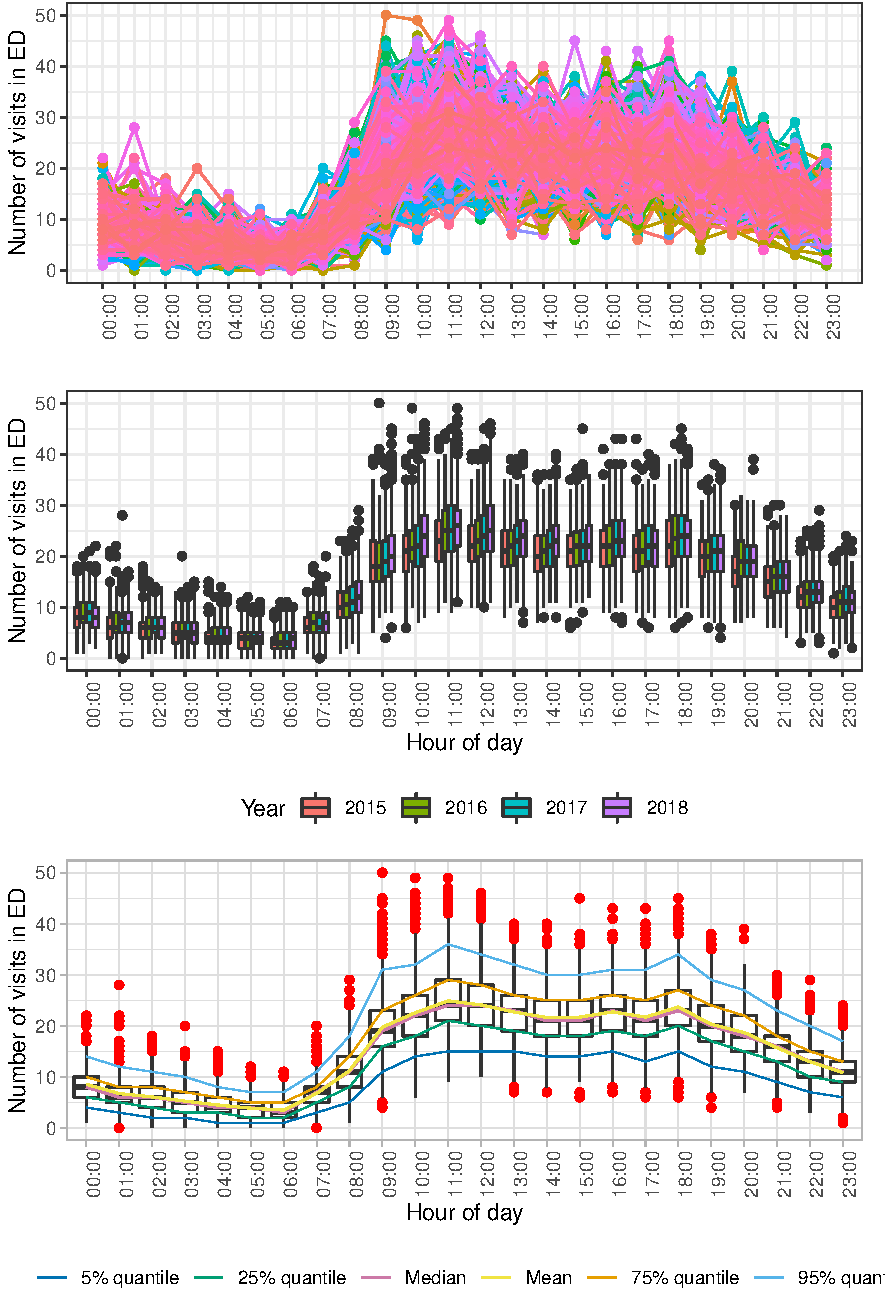
\includegraphics[width=0.8\linewidth]{paper_files/figure-latex/hourly-plot-1} 

}

\caption{Seasonal plot of ED attendance}\label{fig:hourly-plot}
\end{figure}

Figure \ref{fig:24hour}

\begin{figure}[H]

{\centering 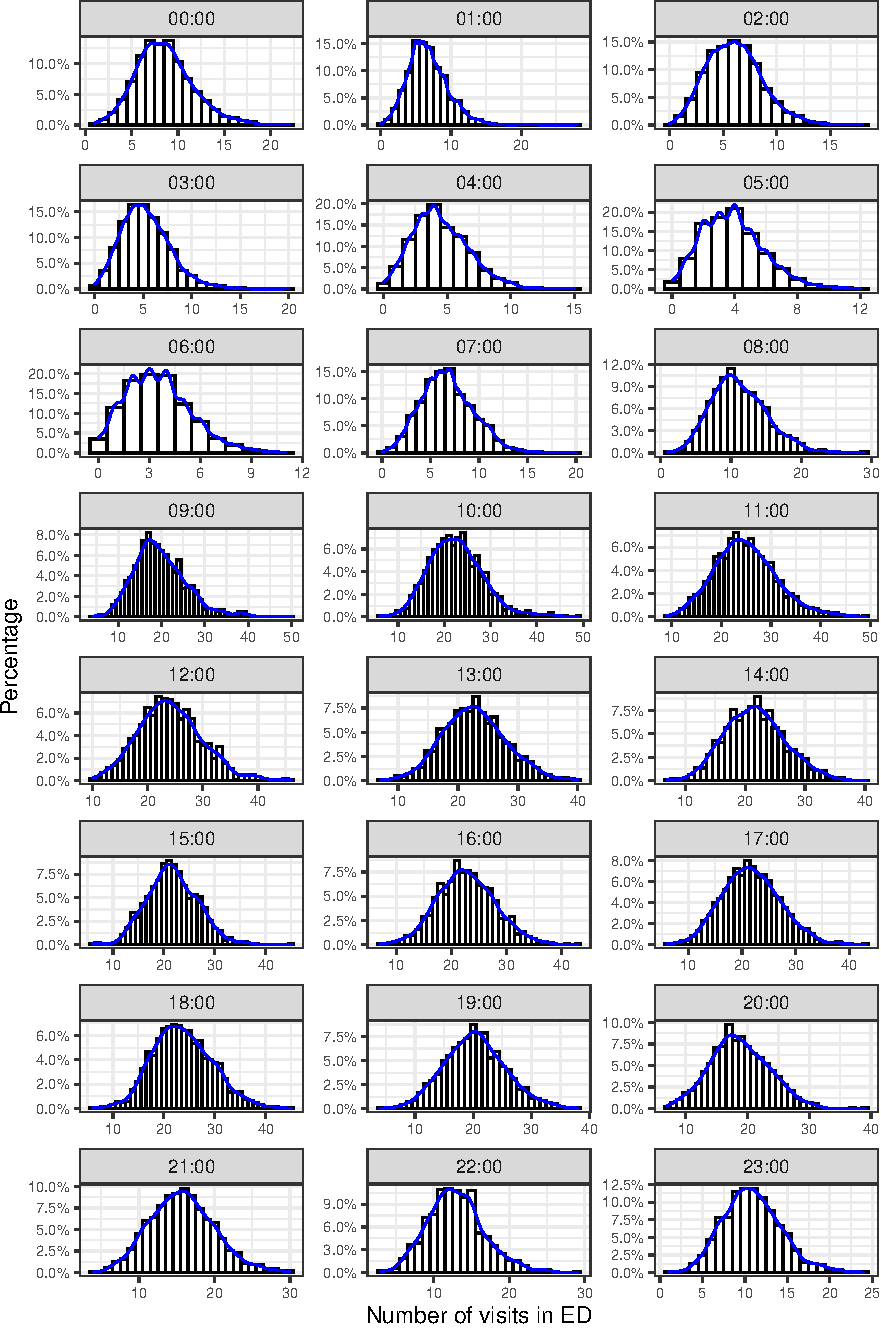
\includegraphics{paper_files/figure-latex/24hour-1} 

}

\caption{Distrubution of ED attendance for each hour of day}\label{fig:24hour}
\end{figure}

\hypertarget{benchmarks}{%
\subsection{benchmarks}\label{benchmarks}}

\begin{equation}
\bar{X} = \frac{\sum_{i=1}^n X_i}{n} \label{eq:mean}
\end{equation}

Also see Equation \eqref{eq:mean}

\hypertarget{accuracy}{%
\subsection{forecast performance evaluation}\label{accuracy}}

\hypertarget{result}{%
\section{Result and discussion}\label{result}}

\hypertarget{conclusion}{%
\section{Conclusion}\label{conclusion}}

\renewcommand\refname{References}
\bibliography{mybibfile.bib}


\end{document}


